\subsection{Gaussian Noise with Salt and Pepper}

By analyzing image 2 in an uniform area it can be seen that the image has both salt and pepper noise, illustrated in figure \ref{fig:hist2_uniform}.
As in section \ref{image_1} this is removed with a shifted median filter. 
It was found that a 5x5 filter removed the extreme values but was not efficient at removing the rest of the noise.

\begin{figure}[H]
\centering
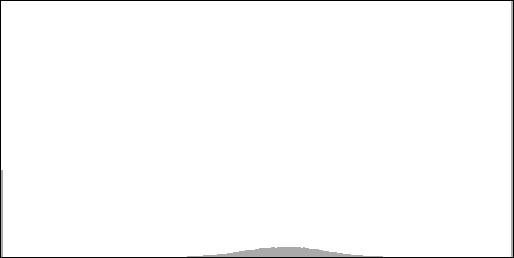
\includegraphics[width = \histogramWidth]{graphics/hist2_uniform.png}
\caption{Histogram of the original ``Image2.png'' showing salt and pepper noise in a uniform area.}
\label{fig:hist2_uniform}
\end{figure}

Thus a harmonic mean filter is used to remove the remaining salt noise.
In figure \ref{fig:hist2_median} can it be seen that the removal of salt and pepper noise was successful.

\begin{figure}[H]
\centering
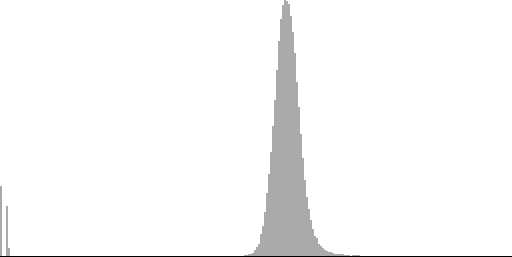
\includegraphics[width = \histogramWidth]{graphics/hist2_after_median.png}
\caption{Histogram of the uniform area after median filter.}
\label{fig:hist2_median}
\end{figure}

Gaussian noise remains and this was removed with a homomorphic bilateral filter.
In figure \ref{fig:hist2_bilateral} can it be seen that the variance has decreased.

\begin{figure}[H]
\centering
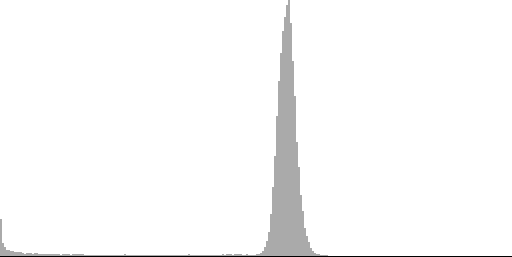
\includegraphics[width = \histogramWidth]{graphics/hist2_after_bilatteral.png}
\caption{Histogram of the uniform area after bilateral filter.}
\label{fig:hist2_bilateral}
\end{figure}

By analyzing a complex region, it can be seen that the image lacks contrast.
In figure \ref{fig:complex2_bilatteral} can the image be seen after a median filter and the homomorphic bilatteral filter.

\begin{figure}[H]
\centering
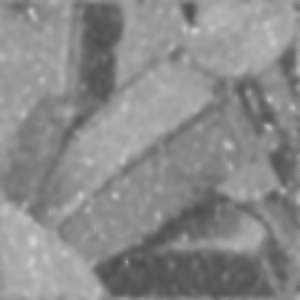
\includegraphics[width = \cutOutWidth]{graphics/complex2_bilatteral.png}
\caption{The complex area after bilatteral filter.}
\label{fig:complex2_bilatteral}
\end{figure}

The lack of contrast can be added with a histogram equalization scheme.
In figure \ref{fig:complex2_histeq} can the image be seen after histogram equalization.

\begin{figure}[H]
\centering
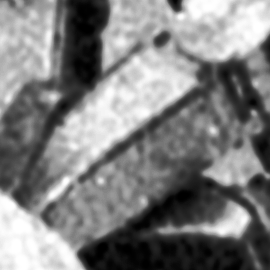
\includegraphics[width = \cutOutWidth]{graphics/complex2_histeq.png}
\caption{Histogram equalization of the complex area.}
\label{fig:complex2_histeq}
\end{figure}


The histogram equalization stretches the color values to the extremes and thus the image quality does not improve.
So before the histogram equalization, a alpha trimmed mean with the kernel size of 7x7 and mean width of 3 is applied to remove further extreme values.
In figure \ref{fig:complex2_histeq_smoothed} can the image be seen after alpha trimmed smoothed and then histogram equalization.

\begin{figure}[H]
\centering
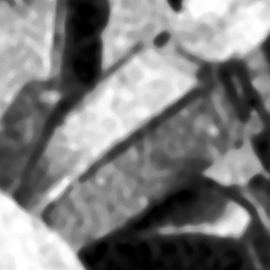
\includegraphics[width = \cutOutWidth]{graphics/complex2_histeq_smoothed.png}
\caption{Histogram equalization of the smoothed compex area.}
\label{fig:complex2_histeq_smoothed}
\end{figure}

The resulting image restoration of image 2 can be seen in figure \ref{fig:image_2_restored}.

\begin{figure}[H]
\centering
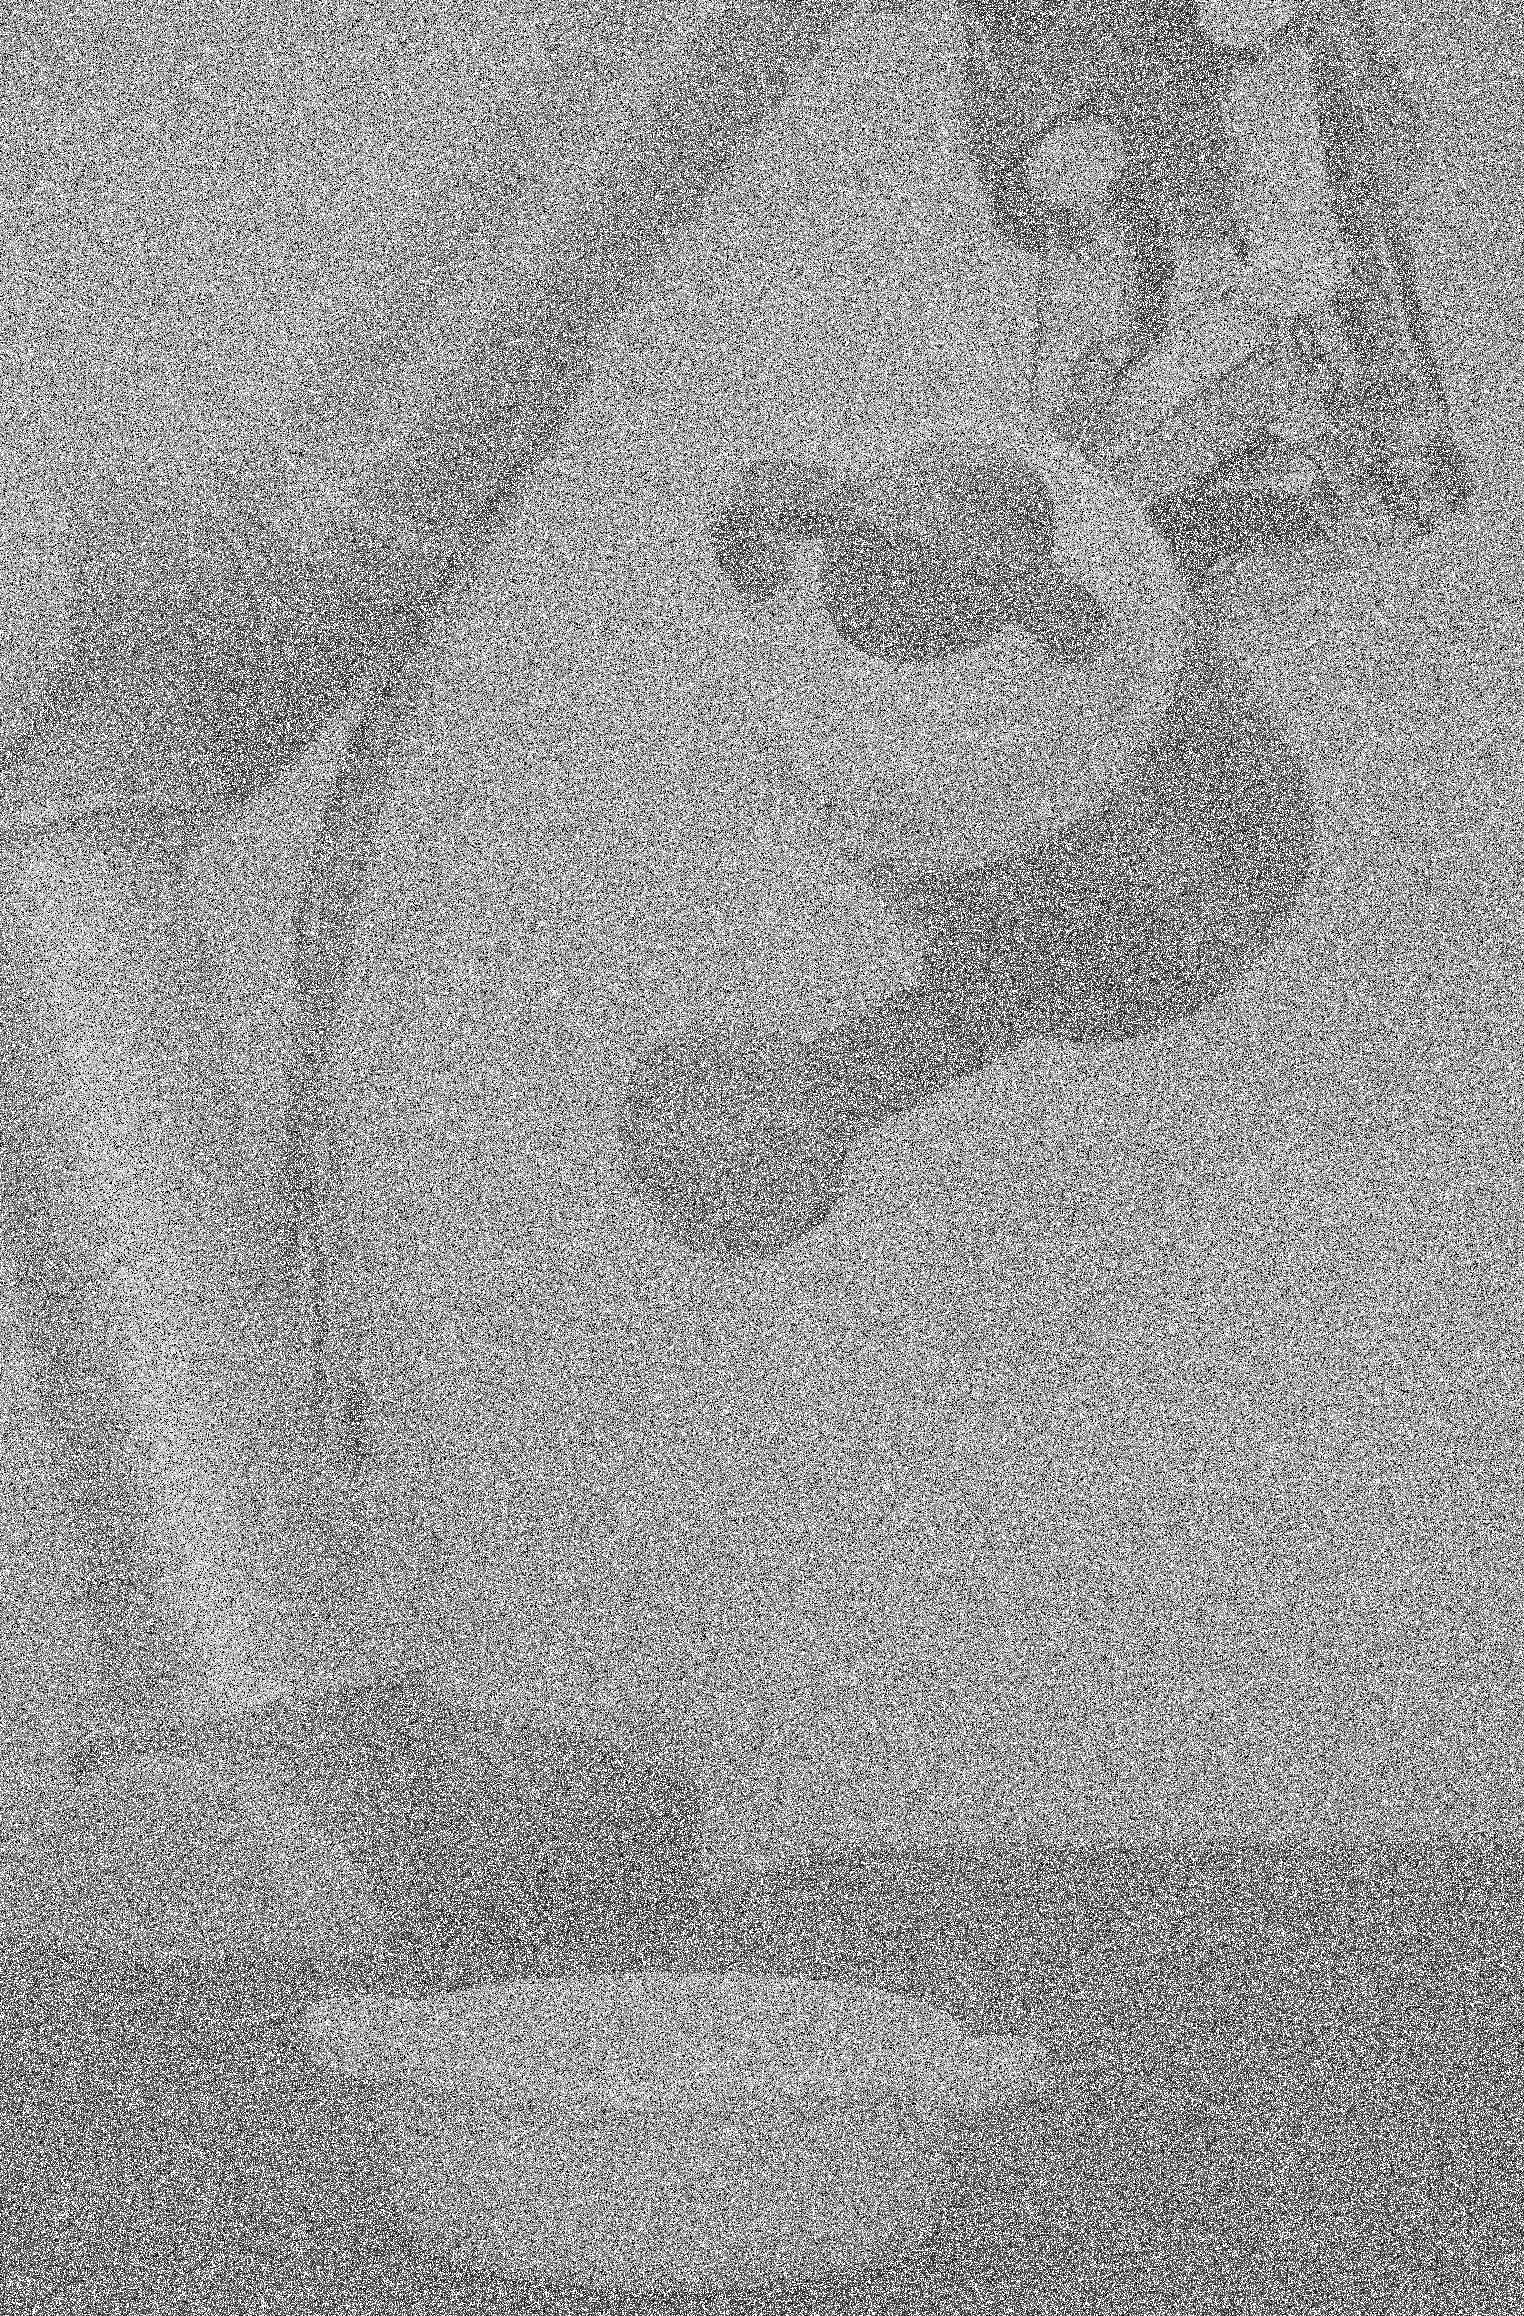
\includegraphics[width = \fullImageWidth]{../code/images/image_result_2.png}
\caption{The restored image 2.}
\label{fig:image_2_restored}
\end{figure}
